\documentclass[a4paper,11pt]{article}
\usepackage[latin1]{inputenc}
\usepackage[spanish]{babel}
\usepackage{bm}
\usepackage{graphicx}
\usepackage{amsmath}
\setlength{\textheight}{235mm}
\setlength{\textwidth}{168mm}
\setlength{\oddsidemargin}{0pt}
\pagestyle{empty}
\begin{document}
	\mbox{}\vspace*{-45mm}
	
	{\centering
		{\small\sc Escuela T�cnica Superior de Ingenieros de Caminos, Canales y
			Puertos (Madrid)}\\*[4mm]
		{\Large\bf M�todo de los Elementos Finitos (Curso 19-20)}\\*[4mm]
		EXAMEN FINAL EXTRAORDINARIO (10 de julio de 2020) \\*[4mm]
	}
	
	\vspace{3mm}
	
	%%%%%
	\paragraph{1.} Se considera una chapa cuyas dimensiones y geometr�a son las indicadas
	en la figura adjunta. Se desea realizar un c�lculo termomec�nico, con el programa FEAP, para conocer las
	cargas que es necesario aplicar en los puntos C y D con el fin de que el movimiento de dichos
	puntos sea nulo.
	La condiciones en los bordes de la chapa se indican en el siguiente cuadro\footnote{En las esquinas en que hay definidas tanto condici�n de flujo como de
		temperatura se impondr� esta �ltima}:
	
	\begin{center}
		\begin{tabular}{|c|l|}
			\hline \hline
			Lado & Condici�n \\ \hline \hline
			$AB$ & $q_n=-250$ W/m$^2$ \\ \hline \hline
			$BC$ & $q_n=-250$ W/m$^2$ \\ \hline
			$CD$ & $383$ $^{\circ}$K \\ \hline
			$DA$ & $180$ $^{\circ}$K \\ \hline
			$EF$ & Aislado           \\  \hline
			$FG$ & Aislado           \\ \hline
			$GH$ & Aislado           \\ \hline
			$HE$ & Aislado           \\ \hline
		\end{tabular}
	\end{center}
	
El coeficiente de conductividad t�rmica es $\lambda=150$ W/(m$\cdot$K).
	
En cuanto a las condiciones de contorno del problema mec�nico, �stas son las
correspondientes a que $AB$ y $AD$ son ejes de simetr�a.

Las propiedades mec�nicas son $E=25$ GPa, $\nu=0.21$,
$\alpha=3.5\cdot 10^{-4}$ $^{\circ}$K$^{-1}$, y
la temperatura de referencia (a la cual las deformaciones t�rmicas son nulas)
es $120$ $^{\circ}$K.. Se considera la
hip�tesis de deformaci�n plana.
	\begin{center}
		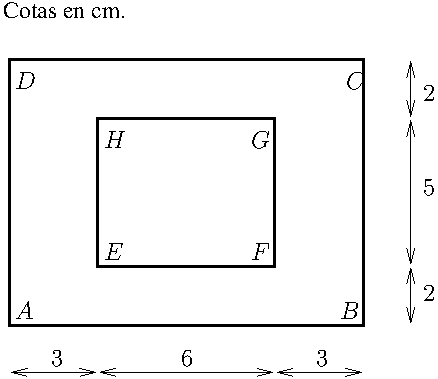
\includegraphics[width=0.35\textwidth]{ej2}
	\end{center}

En el caso de que en $C$ y $D$ se han aplicado las cargas necesarias para que no se muevan,
se pide subir los siguientes ficheros de resultados:
\begin{enumerate}
	\item Fichero de entrada de datos de feap
	\item Contornos de movimientos horizontales
	\item Contornos de movimientos verticales
	\item Escribir en la tarea creada a tal efecto los valores obtenidos de la carga vertical que
	es necesario aplicar en $D$  y las cargas horizontal y vertical que hay que aplicar en $C$ para que estos puntos no se muevan.
\end{enumerate}
	
	{\em NOTAS:}
	\begin{itemize}
		\item La malla estar� formada por elementos cuadrados de lado $0.2$ cm
		\item En los puntos singulares en los que hay una condici�n de flujo y
		temperatura impuestos de forma simult�nea, se considerar� la condici�n de
		temperatura impuesta.
		\item En el v�rtice $D$ la temperatura a considerar es $180$ $^{\circ}$K
	\end{itemize}
	
\end{document}

